\section{A General Overview of Kalman Filtering}
Kalman Filters (KF) fall under the umbrella of Machine Learning models, however are additionally an example of a mechanistic model. This results in being able to tune pieces in the Kalman Filtering algorithm rather than being left to deal with a black box. Moreover, unlike MCMC's, which are used on already corrected data sets, Kalman Filters can be adjusted as new data is brought in. Rather than making predictions using an entire dataset at once, KFs improve and evolve as more datapoints are assessed. To use a KF, you must put your model into a discretized state space form. To do this, you must identify two sets of variables: latent states and observables. Latent states are the set of variables that one is interested in estimating, which can include values such as a population count or model parameters. On the other hand, observables are a set of data which has been measured from the system and is the only piece of information known about the system at a particular time point. Additionally, Kalman Filters are helpful due to their ability to quantify the noise associated with a system. This is achieved through both process and measurement noise. Process noise describes outside forces and situations which, as a result of their actions, affect states in the model. Measurement noise, on the other hand, accounts for the fact that tools to gather observable data may be inherently flawed, and thus some level of noise is associated with the values they produce. In order to gather a holistic, high level understanding of Kalman Filters, consider the example of a car driving down a street.\\
\\
Assume that one observes a car at time $t$ traveling at a velocity of 5 m/s at a position of 2 m from an observed starting point. In order to estimate what the car's velocity will be at time $t+1$, one may choose to utilize a Kalman Filter. Assuming that the position at time $t+1$ can be measured to be 5 m with a device, this position thus is the observable, while the velocity is a latent state. However, since the tool is flawed, measurement noise is added in as well. If we assume that while this is occurring, a 25 mph wind blows from behind the car, this would now become a source of process noise. Having all of this information, one is now capable of applying a KF to estimate the velocity of the car at time $t+1$.\\
\\
Kalman Filters operate in discrete time, state space models, meaning that we have input and output variables being related to one another through a system of ODEs at known time points. Thus, we must have knowledge about the system to the extent that we know the structure of the ODEs, although as we'll see, there are formats of the Kalman Filter in which it is not necessary to know the parameter values. Having both an understanding of the ODEs and the observable data, we can now introduce the the projection and update steps, the two of which drive the KF algorithm. 
%{The simplest use of Kalman Filters is for state estimation, which we will describe in the following sections. Although our eventual goal is to implement parameter estimation, since parameter estimation is based on the foundation of state estimation, it is easier to understand if you first have a general understanding of state estimation. As a result of this, we will introduce  parameter estimation later on.%} 
\subsection{Projection Step}
The first step of the KF relies only on knowledge of the system. Having an estimate of latent states at time $t$, we use our knowledge of the system to predict the states at time $t + 1$, known as the prior estimate.
\subsection{Update Step}
Having a prior estimate, we can now bring in the observable data. By seeing how the prediction we made in the Projection Step compares to the observable data, we now update our predictions and states. This is now our posterior estimate, and becomes the set of states that are projected forward to produce the prior estimate for time $t+2$. We continue this loop as long as new data is coming in, continously improving results as more data arrives. Figure X shows this two step process visually, as we continously iterate over the two steps are more data is available. \\
\\
\begin{figure}[H]
    \centering
    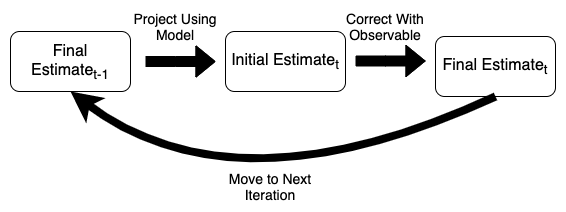
\includegraphics[width=15cm]{Kalman Filter Images/Kalman_Filter_Simple_Diagram.png}
    \caption{The two steps of the Kalman Filter algorithm. First, we use knowledge of the system to create an initial prediction, following which observable data is produced to produce final estimates.}

\end{figure}

\section{Introduction to Kalman Filters}

    \subsection{Different Types of Kalman Filters}
    There are multiple types of Kalman Filters, for different types of systems. When a system is linear, one may use the standard Linear Kalman Filter. However, once the system becomes nonlinear this is no longer feasible. If the nonlinear system may be accurately linearized with first order Taylor approximations, the Extended Kalman Filter (EKF) may be used, the theory for which is based around this Taylor approximation. However, if the nonlinear system  is not easily linearized, it is recommended to use the Unscented Kalman Filter (UKF). Due to the inability of complex ODE systems to be accurately approximated with first order Taylor approximations, we will focus on the Unscented Kalman Filter.
    
    \subsection{Process and Measurement Equations}
    The Unscented Kalman Filter is used to estimate the states of a nonlinear system. The system, set up as a state space model, is described by the process and measurement equations. The process equation, describing the transition of the latent states from time $k$ to time $k+1$ is formulated as
    $$x_{k+1} = F_{k+1,k}(x_k) + q_k \ (1.1)$$
    where $x_{k}$ is the vector of states at time $k$, $x_{k+1}$ is the vector of states at time $k+1$, $F$ is the non-linear transition function that takes the state from time $k$ to time $k+1$, and $q_k$ is the process noise. $F$ and $q_k$ are assumed to be known quantities. The Measurement equation, describing the relationship between observed data points and the unknown states, is 
    $$y_k = H_k(x_k) + r_k \ (1.2)$$
    where $y_k$ is the vector of the observables, $H$ is a (possibly) nonlinear function that relates the states to the observables, and $r_k$ represents the measurement noise. $H$ and $r_k$ are assumed to be known. 
    \subsection{Set up of the Noise}
    The above system of equations relies on both process and measurement noise. The vector $q_k$, which follows the same dimensions as the state vector in order to apply one noise value to each state, describes the process noise and is multiviate Gaussian with mean 0 and covariance described by
    $$E[q_{n}q_{k}^T] = \Bigg\{\begin{tabular}{l}
    $Q_k$\ for\ n = k  \\
    0   for \ $n \neq k$
    \end{tabular} (1.3)$$
    
    Similarly, $r_k$ describes the measurement noise and is Gaussian with mean 0 and covariance described by
    $$E[r_{n}r_{k}^T] = \Bigg\{\begin{tabular}{l}
    $R_k$\ for\ n = k  \\
    0   for \ $n \neq k$
    \end{tabular} (1.4)$$
    
    
    Both of these covariance matrices will play a role in the UKF calculations. Furthermore, it is important to note that our system assumes white, additive noise. If we have a system where the noise isn't additive, we must set up the UKF slightly differently (CITATION FOR OTHER SET UP). 
    
    \subsection{Unscented Transformation}
    The Unscented Kalman Filter is formulated around the Unscented Transformtation (UT). The UT is used to understand the distribution of a random variable after a nonlinear transformation has been applied to it. Consider random variable $x$ with dimension $L$ and nonlinear function $y = f(x)$. Assume that $\bar{x}$ is the mean of the distribution of $x$ and $P_x$ is the covariance of the distribution of $x$. To understand distribution of the nonlinear transformation y, we create matrix $\chi$ of 2$L$ + 1 sigma vectors as follows:
    $$ \chi_0 = \bar{x}$$
    $$ \chi_i = \bar{x} + (\sqrt{(L + \lambda)P_x})_i \ i = 1 ... L  \ (1.5)$$
    $$ \chi_i = \bar{x} - (\sqrt{(L + \lambda)P_x})_{i - L} \ i = L + 1 \  ...  \ 2L + 1 $$
    The number 2$L$+1 gives us one vector at the mean, and $L$ vectors above and below the mean. As stated above, $L$ is the dimension of $x$ which means it is number of states in our system. The subscript $i$ refers to the $i$th columns in the matrix square root of the term $(\sqrt{(L + \lambda)P_x})$.
    Here, $\lambda$ is a final scaling parameter defined as $\alpha^2(L + k) - L$, where $\alpha$ is a scaling parameter that represents the spread of vectors around $\bar{x}$. $k$ is a secondary scaling parameter, set to either 0 or $3-L$, whereas $\alpha$ takes on a value between 10e-4 and 1 (ADD WAN MERE CITATION HERE). It is crucial to note that this is a form of \textbf{deterministic} scaling. In many sampling schemes, sampling is done \textbf{randomly} from a distribution. However, here our goal is to choose points in equal intervals and in equal quantities of either side of the mean, $\bar{x}$. The purpose of this is so that we may be certain that sigma points accurately capture the spread of a distribution. With random sampling, if only choosing a small amount of points, we can make no guarantees about the distribution of these points. Thus, exact equations are given for how the sigma points should be chosen. \\
    \\
    Once $\chi$ has been calculated, the sigma points are then sent through the nonlinear function $f$ to create vectors $Y_i$. This is done as follows:
    $$Y_i = f(\chi_i) \ \ i = 0,...,2L \ (1.6)$$
    
    As we will soon see, in the context of the UKF, the Unscented Transformation is used to both understand the prior estimate $\hat{x}^-$ (when $F$ plays the role of $f$ here) and the predicted observable values $\hat{y}_k^-$ (when $H$ plays the role of $f$ here).\\
    \\
    Now, by weighting these output vectors $Y_i$ in a deterministic fashion, we can calculate a mean and covariance in order to understand our new distribution. In order to do this, we create the following weights, where $W^{(m)}$ are weights corresponding to calculating the mean and $W^{(c)}$ is used to calculate our covariance:
    $$ W_0^{(m)} = \lambda/(L + \lambda)  \ (1.7)$$ 
    $$ W_0^{(c)} = \lambda/(L + \lambda) + (1 - \alpha^2 + \beta) \ (1.8) $$
    $$ W_i^{(m)} = W_i^{(c)} = 1/{2(L + \lambda)} \ i = 1 ... 2L \ (1.9) $$
    Here, $\beta$ holds prior knowledge about the distribution (for Gaussian $\beta = 2$ is used). We can see that the sigma point that represents the mean is given more weight than the others. Now the mean and covariance can be calculated:
    $$ \bar{y} \approx \sum_{i = 0}^{2L} W_i^{(m)} Y_i \ (1.10)$$
    $$ P_y \approx \sum_{i = 0}^{2L} W_i^{(c)}(Y_i - \bar{y})(Y_i - \bar{y})^T  \ (1.11)$$
    Understanding this mean and covariance will be useful in creating our prior estimates in the UKF method.
    \\
    \\
    For a visual representation, see the figure below from WanMere Chapter 7 (CITATION):\\
    \begin{figure} [H]
    \centering
    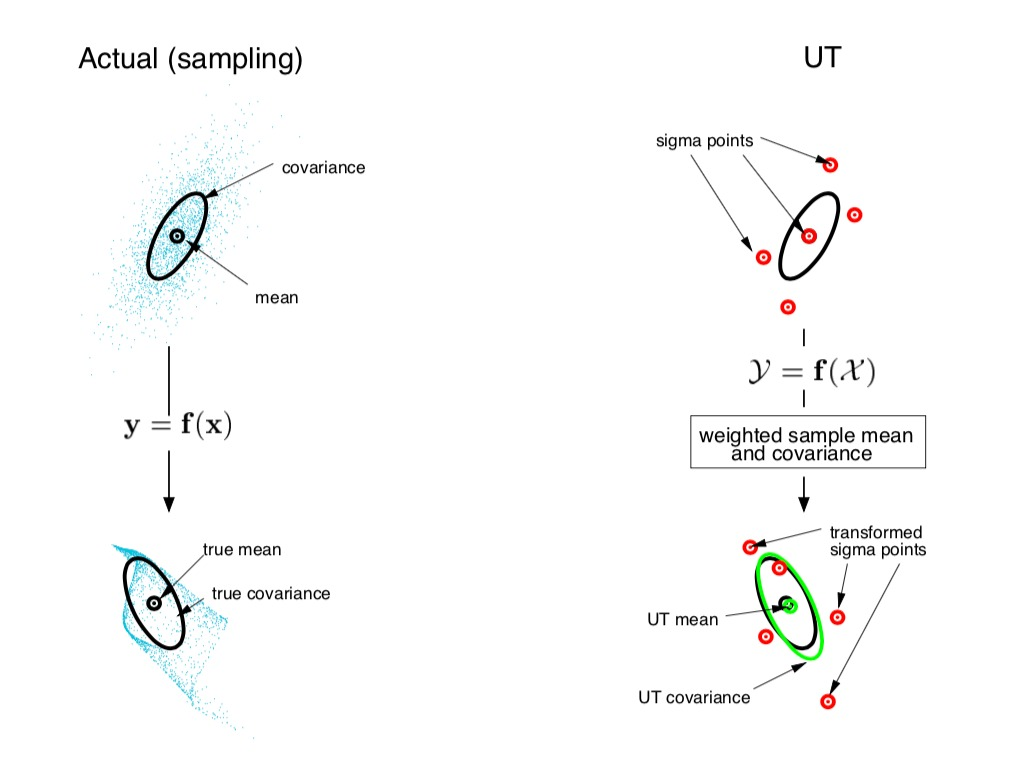
\includegraphics[scale = .5]{Kalman Filter Images/Chapter7ImageUpdated.jpg}
    \caption{A figure from WanMere Chapter 7 comparing the Unscented Transformation (right) with a standard sampling procedure (right). The UT, due to its use of Sigma Points, is able to accurately capture the distribution following the nonlinear transformation $y$.}
    \end{figure}
    Here, on the left hand side is what the nonlinear transformation on the data $x$ through the function $f(x)$ ideally looks like (i.e. when all the values are known). On the right, using the Unscented Transformation (UT), we now instead create a sample of points from the distribution (sigma points), and apply the transformation to them. The sigma points that are chosen are indicated by the red circles. Then, using a weighting schema, we find a sample mean and covariance for the points after they have  gone through the nonlinear transformation. We can see that the Unscented Transformation process, even though it only uses a select number of points, is able to accurately capture the true mean and covariance as presented on the left. 
    
    \section{Kalman Filter Description}
    
    \subsection{Notation}
    Before going deeper into the process of using a Kalman Filter, it is important to establish the notation that will be used throughout. 
    \subsubsection{States Notation}
    For our states, we have $\hat{x}_0$, our very first posterior estimate. Next, we notate our prior estimate as $\hat{x}_k^-$ and our posterior estimate, following the Update Step, as $\hat{x}_k$. Then, we have analogous notation for the states covariance. Namely, we start with $P_0$, have a prior estimate of $P_k^-$, and then a posterior covariance of $P_k$.
    \subsubsection{Observables Notation}
    We must define similar notation for our observables. Here, we have a prior estimate $\hat{y}_k^-$, but instead of a posterior estimates, we have the \emph{actual} observable value $y_k$. Using these two values, we also define the error, or \emph{innovation}, as:
    $$\tilde{y}_k = y_k - \hat{y}_k^-$$
    Then, we once again have a covariance matrix, but this time for the innovation, $P_{\tilde{y}_k}$. This is the basis of the notation, however more will be introduced as necessary in the following sections, and a full guide can be found in table X (NEED TO MAKE THIS TABLE OF ALL NOTATION!!!)
    
    \subsection{Initialization}
    The initial states vector $x_0$ and the initial covariance matrix between the states, $P_0$, are needed to initialize the UKF. To create these initial guesses some prior knowledge of the states and their plausible ranges is necessary. Assuming this information is available, one may initialize with:
    $$\hat{x}_0 = E[x_0] \ (1.12)$$
    and initial covariance matrix:
    $$P_0 = E[(x_0 - \hat{x}_0)(x_0 - \hat{x}_0)^T] \ (1.13) $$
    When working with real data, one is not likely to have a full understanding of the states' distribution. Thus, a first guess will suffice and may be tuned throughout working with the UKF, as will be discussed in the \textbf{Kalman Filter Implementation} section.  
    \subsection{Projection Step}
    Now, we proceed to do the projection portion of the algorithm. Having chosen a set of sigma points via  equations (1.5), we now project them in time by applying the transition matrix to each point in the vector $\chi_{k-1}$:
    $$\chi_{k|k-1} = F(\chi_{k-1}) \ (1.14)$$
    It is important to note that here $\hat{x}_{k-1}$ plays the role of $\bar{x}$ in (1.5).
    Next we calculate a prior prediction of the state $\hat{x}_k^-$ with:
    $$ \hat{x}_k^- = \sum_{i = 0}^{2L} W_i^{(m)} \chi_{i, k|k-1} \ (1.14)$$
    Similarly we can calculate a prior covariance $P_k^-$ by using our weights as well as the process noise:
    $$ P_k^- = \sum_{i = 0}^{2L} W_i^{(c)} [\chi_{i, k|k-1} - \hat{x}_k^-][\chi_{i, k|k-1} - \hat{x}_k^-]^T + Q \ (1.15)$$
    We can see that the calculation of $\hat{x}_k^-$ and $P_k^-$ are both applications of the Unscented Transformation. Next, we apply the UT transformation to understand our observables with:
    $$ Y_{k|k-1} = H[\chi_{k|k-1}] \ (1.16)$$
    This allows us to know calculate a prior estimate of the observables $y_k^-$ by utilizing:
    $$ \hat{y}_k^- = \sum_{i=0}^{2L} W_i^{(m)} Y_{i,k|k-1} \ (1.17) $$
     Once again, we have made use of the UT transformation here.
    \subsection{Update Step}
    Having created prior estimates for both states and observables, we now proceed to the update step where the observed data is brought in. \\
    \\
    We begin by calculating the covariance matrix $P_{\tilde{y}_k, \tilde{y}_k}$, which is the covariance matrix for the error between the projected and actual values of the observables. We denote this error value as 
    $$\tilde{y}_k = y_k - \hat{y}_k^-$$
    This quantity is also known as the \emph{innovation} and represents how far off our estimate of the observable is from the true value.\\
    \\
    Moreover, this calculation takes into account the measurement noise through $R$:
    $$ P_{\tilde{y}_k, \tilde{y}_k} = \sum_{i=0}^{2L} W_i^{(c)} [Y_{i,k|k-1} - \hat{y}_k^-][Y_{i,k|k-1} - \hat{y}_k^-]^T + R \ (1.18)$$
    Next we need a covariance between our states and observables, which is calculated by:
    $$ P_{{x}_k,{y}_k} = \sum_{i=0}^{2L} W_i^{(c)} [\chi_{i,k|k-1} - \hat{x}_k^-][Y_{i,k|k-1} - \hat{y}_k^-]^T \ (1.19)$$
    At this point, we have sufficient information to calculate the \textbf{Kalman Gain}, a crucial term in the UKF algorithm. The Kalman Gain is used to weight the error between the predicted value and the observed value of $x_k$ in order to update the filter's prior predictions. A larger Kalman Gain will give more weight to the error, resulting in a larger correction and a smaller Kalman Gain will give less weight to the error, resulting in a smaller correction. The Kalman Gain is also used to adjust the covariance matrix $P_k$ and is calculated through:
    $$K_k = P_{x_k, y_k} P_{\tilde{y}_k, \tilde{y}_k}^{-1} \ (1.20) $$
    Calculation of the Kalman Gain allows us to calculate our posterior estimates of both the states, $\hat{x}_k$, and covariance, $P_k$. For the states the following equation is used
    $$\hat{x}_k = \hat{x}_k^- + K_k(y_k - \hat{y}_k^-) \ (1.21)$$
    And for the covariance we use:
    $$ P_k = P_k^-  - K_k P_{\tilde{y}_k, \tilde{y}_k} K_k^T \ (1.22)$$
    We can see that both equations function by adjusting our prior prediction through use of the Kalman Gain.\\
    \\
    After having gone through the update step, the next data point would be brought in and we would return to the Projection Step once more.
    \subsection{Summary}
    A flow chart depicting one iteration of the entire UKF process is below. To summarize, our goal is to begin with a set of sigma points chosen in a deterministic fashion and arrive at the posterior estimates for the states and covariance. This is done in two main sections, the Projection Step, whose quantities are shaded in red, and the Update Step, displayed in blue.
    
    \begin{figure} [H]
    \centering
    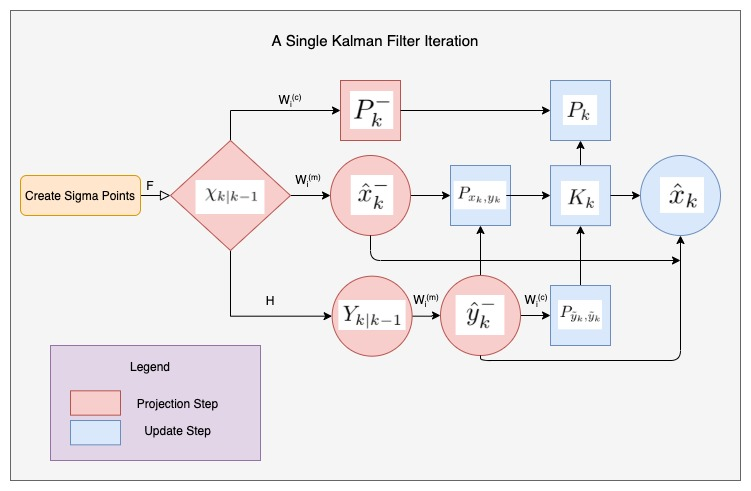
\includegraphics[scale = 0.6]{Kalman Filter Images/UKFFlowDiagram.jpg}
    \caption{A flow chart depicting one iteration of the UKF process. The sigma points are shaded in yellow, the intermediate steps in red, the Kalman gain in green, and the posterior estimates in blue.}
    \end{figure}
    
    \subsection{Stability and Divergence Issues}
    When utilizing the UKF, it is important to consider the issue of positive definitiness of the covariance matrix $P_k$. If this matrix becomes non-positive definite, the filter can experience severe divergence issues due to invalid covariance matrices, which can occur as a result of the update made in (1.22), due to the covariance to becoming non positive-definite. This then can lead the filter to diverge.  (ADD CITATION). \\
    \\
    The solution to the issue lies in using the \textbf{Cholesky factorization}.
    \\
    \\
    At every iteration of the Kalman Filter, one must perform the following step:
    $$P_k = {P_k}^{1/2} {P_k}^{T/2}$$
    Where ${P_k}^{1/2}$ is the \textbf{Cholesky factor} and is in lower-triangular form, and ${P_k}^{T/2}$ is the Cholesky factor's transpose. Here, $P_k$ is now the product of a square matrix and its tranpose, which is \textbf{guranteed to be positive definite}. In order to find the Cholesky factor, a function such as Matlab's \emph{chol} (https://www.mathworks.com/help/matlab/ref/chol.html) can be used. By using this approach, one will have a better chance of maintaining the stability of the Kalman Filter across iterations.\\
    \\
    
    
    
\begin{tcolorbox}
\doublespacing
\textbf{\underline{The Unscented Kalman Filter Algorithm With Additive Noise}} 
\begin{enumerate}
    \item Initialize $\hat{x}_0 = E[x_0]$ or with best guess.
    \item Initialize $P_0 = E[(x_0 - \hat{x}_0)(x_0 - \hat{x}_0)^T]$ or with best guess.
    \item For each incoming data point perform the following:
    \begin{enumerate}
        \item Projection Step
        \begin{enumerate}
            \item Create Sigma Points 
            \begin{itemize}
                \item  $\chi_0 = \bar{x}$
                \item $ \chi_i = \bar{x} + (\sqrt{(L + \lambda)P_x})_i \ i = 1 ... L $
                \item $ \chi_i = \bar{x} - (\sqrt{(L + \lambda)P_x})_{i - L} \ i = L + 1 \  ...  \ 2L + 1 $
            \end{itemize}
            \item Project Sigma Points forward with $\chi_{k|k-1} = F(\chi_{k-1})$
            \item Calculate prior state estimate $ \hat{x}_k^- = \sum_{i = 0}^{2L} W_i^{(m)} \chi_{i, k|k-1}$
            \item Calculate prior covariance estimate $ P_k^- = \sum_{i = 0}^{2L} W_i^{(c)} [\chi_{i, k|k-1} - \hat{x}_k^-][\chi_{i, k|k-1} - \hat{x}_k^-]^T + Q$
            \item Project observables forward with $Y_{k|k-1} = H[\chi_{k|k-1}]$
            \item Calculate prior observable estimate $\hat{y}_k^- = \sum_{i=0}^{2L} W_i^{(m)} Y_{i,k|k-1}$
        \end{enumerate}
        \item Update Step
        \begin{enumerate}
            \item Calculate innovation covariance $P_{\tilde{y}_k, \tilde{y}_k} = \sum_{i=0}^{2L} W_i^{(c)} [Y_{i,k|k-1} - \hat{y}_k^-][Y_{i,k|k-1} - \hat{y}_k^-]^T + R$
            \item Calculate state and observable covariance $ P_{{x}_k,{y}_k} = \sum_{i=0}^{2L} W_i^{(c)} [\chi_{i,k|k-1} - \hat{x}_k^-][Y_{i,k|k-1} - \hat{y}_k^-]^T$
            \item Calculate Kalman Gain $K_k = P_{x_k, y_k} P_{\tilde{y}_k, \tilde{y}_k}^{-1}$
            \item Calculate posterior state estimate $\hat{x}_k = \hat{x}_k^- + K_k(y_k - \hat{y}_k^-)$
            \item Calculate posterior state covariance $P_k = P_k^-  - K_k P_{\tilde{y}_k, \tilde{y}_k} K_k^T$
            \item Perform Choletsky Factorization $P_k = {P_k}^{1/2} {P_k}^{T/2}$
        \end{enumerate}
        \item Set $k$ to $k + 1$ and proceed to next data point
        
        \end{enumerate}
    \end{enumerate}


\end{tcolorbox}
\singlespacing    
    
    
    
\section{Parameter Estimation - Dual versus Joint}
Up to this point the UKF has been described in the sense of performing state estimation, where the parameters of the ODE model are known in full. However, there are often scenarios, such as the Lotka-Volterra and T1D systems, where model parameters are unknown and need to be estimated. In order to do so, we can use the Joint and Dual UKF methods.

    \subsection{Joint}
    The Joint UKF algorithm is done very similarly to a standard state-estimation UKF. However, the parameters of the model, call them $\theta$, are now added to the state vector to make one large state vector. In essence, the parameters become states to be estimated. Thus, given states $x$ and parameters $\Theta$, our latent states vector becomes a concatenation of the two. In order to implement this, we treat the transition function related to the parameters as an identity since our goal is to estimate constant parameter values.
    
    \subsection{Dual}\\
    In the Dual UKF, two UKFs are run in parallel, one for the states and one of the parameters. The estimates for the parameters at a specific time point are then fed into the state filter, and the estimates for the states are then fed into the filter for the parameters. Thus, during implementation, two UKF functions are required, one for states and another for parameters. Once again, the transition function for the parameters should be set to an identity matrix.\\
    
The details of these two implementations are discussed in the following portion of this work.